\chapter{Introduction}
\label{c:intro}
    Advances in 3D scanning technology and 3D modeling
    techniques have lowered the barrier in creating
    high-resolution 3D models.  
    High-resolution 3D models can now be created
    with laser scanner and reconstruction software.
    For example, the Stanford's Digital Michelangelo Project
    has digitalized several famous statues of Michelangelo
    \cite{levoy00digital} (See Figure \ref{f:intro:scanner}). 
    Similar projects include 
\begin{figure}[htbp!]
\centering
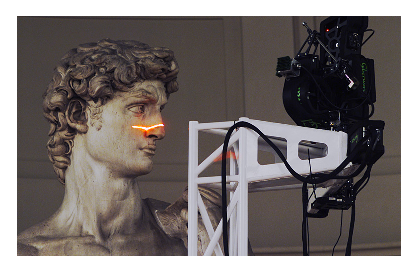
\epsfig{file=scanner.eps, height=0.3\textwidth}
\caption{Stanford's Digital Michelangelo Project. The head of David Statue is being 
scanned (image source: http://graphics.stanford.edu/projects/mich).}\label{f:intro:scanner}
\end{figure}
    the Digital Sculpture Project \cite{deroos2004dsp}
    and the project to digitize Rodin's sculptures \cite{miyazaki2006dab}. 
    Further, artists can directly create high-resolution 3D models with
    digital sculpture softwares such as ZBrush (See Figure \ref{f:intro:zbrush}).
\begin{figure}[htbp!]
\centering
\begin{tabular}{cc}
\epsfig{file=zbrush1.eps, height=0.3\textwidth}
&
\epsfig{file=zbrush2.eps, height=0.3\textwidth}
\end{tabular}
\caption{Complex digital sculptures created with ZBrush
(image source: http://www.evermotion.org/vbulletin/showthread.php?t=64128).}\label{f:intro:zbrush}
\end{figure}

    Sharing high-resolution 3D models over the Internet is useful in many
    applications. Digital museum exhibiting 3D models of artifacts
    is one of the applications. For example, Dr. Andre Stork and his teams are working
    on a project named ``History in 3D''\footnote{
    http://www.fraunhofer.de/en/press/research-news/2009/11/history-in-3d.jsp.}. 
    Exhibiting high-resolution 3D models of artifacts instead of the
    artifacts themselves has many advantages. 
    People can view the artifacts from
    anywhere, at anytime, and without any travel cost. 
    Visitors can interact with exhibited artifacts
    in any way they want, without worrying about damaging them 
    or interfering other visitors. 
    Moreover, the museum can exhibit artifacts, however precious they are, 
    safely without worrying about corrosion and theft.


    High-resolution 3D models are useful in other networked applications too. 
    For example, virtual world applications,
    such as Second Life, can become more realistic and interesting by
    supporting high-resolution 3D models. 
    Commercial users could show their products as 3D models to potential users all over 
    the world. Sculptors could demonstrate their artworks freely without renting an gallery.
    As another example, virtual earth applications, 
    such as Google Earth, could represent many landmark buildings or statues
    (e.g. Statue of Liberty) as high-resolution 3D models to
    give more realistic representation of the real world.

    When used in networked applications, 
    high resolution 3D models may take long time to download completely
    for display at the client. 
    For example, the Stanford model of the David statue, with 28 million vertices and
    56 million triangles, is still 70 MB in size with
    state-of-the-art compression \cite{alliez2001progressive} and needs around 10 minutes
    to download at 1 Mbps.  
    To reduce the waiting time of the user, 
    streaming techniques can be used to transmit 3D models. 
    The 3D streaming technology enables users to render the a coarse version of the model
    based on partially received data as a preview, 
    and then improve the quality when more data becomes available. 
    Users can decide how much data to receive based on their requirement of quality
    and the rendering ability of their hardware.

\begin{figure}[htbp!]
\centering
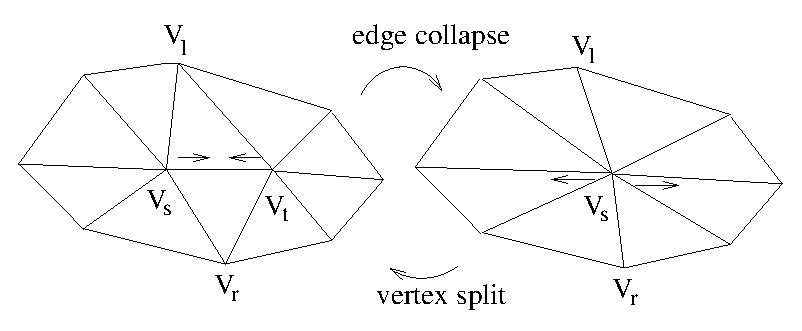
\epsfig{file=split2.eps, width=0.5\textwidth}
\caption{Edge collapse and vertex split}\label{f:intro:split2}
\end{figure}
    One popular representation to support 3D streaming, \textit{progressive mesh}, 
    is proposed by Hoppe \cite{hoppe96progressive}.
    The technique is based on an
    operation called \textit{edge collapse}, and its reverse
    operation, \textit{vertex split}.  Given a (non-progressive)
    3D mesh, the technique applies a series of edge collapses,
    simplifying the model by reducing the number of vertices and
    faces.  The final, simplified model obtained after this
    process becomes the \textit{base model}.  Given a base model,
    we can reconstruct the original model by reversing
    the edge collapse operations through \textit{vertex splits},
    incrementally adding new vertices and faces. So, a
    progressive mesh can be represented by the base
    model and a series of vertex splits.  
    Figure~\ref{f:intro:split2} illustrates edge
    collapse and vertex split operations.
    Progressive streaming can be implemented by sending the base mesh
    first as a preview and then sending vertex splits to improve 
    the quality incrementally (See Figure \ref{f:intro:progressive}).
    \begin{figure}[htbp!]
    \centering
    \epsfig{file=progressive.eps, width=0.85\textwidth}
    \caption{
    Progressive 3D mesh streaming. The original Happy Buddha mesh 
    courtesy of Stanford Computer Graphics Laboratory.
    \label{f:intro:progressive}}
    \end{figure}
    
    Although audio and video streaming have been studied extensively, 
    3D streaming remains a new research topic. 
    Video streaming and 3D streaming are significantly different
    due to the difference between videos and 3D models, and
    the main difference is how users consume the data.
    In video streaming, usually the data are consumed in time order. 
    Whereas in 3D streaming, especially when high-resolution 3D models are used,
    users may consume different subset of the data, and in various orders.
    
    This flexibility is important in streaming of high-resolution 3D models, 
    because streaming a huge 3D model in a fix order leads to transmission of data not
    useful to the user, wasting time and bandwidth.
    Ensuring this flexibility in streaming system is an important consideration
    in choosing representation and coding schemes. The details are discussed
    in Chapter \ref{c:related}.
    Meanwhile, this flexibility introduces some new research questions, 
    which we introduce in the next section. 

  \section{Research Objectives and Scope}
  \label{s:intro:objectives}
    \subsection{Quantitatively Determining the Effect of Dependency}
    In progressive streaming, the quality of the mesh on the receiver
    increases over time.
    Because vertex splits contribute differently to the quality, 
    how quality improves
    depends on the decoding order of the vertex splits,
    which in turn depends on the sending order of the vertex splits.
    Because of the flexibility in choosing sending order,
    it is possible to choose a sending order so that the 
    quality on the receiver increases as fast as possible.

    A natural method is to send vertex splits in the descending order
    of their contribution to the quality of the received mesh. 
    This strategy, however, is not always optimal 
    when the mesh is transmitted over a lossy network,
    because dependency also plays an important role in choosing sending order.
    
    The progressive coding of meshes introduces dependencies among 
    the vertex splits, and the descendants cannot be decoded
    before their ancestors are all decoded. Therefore, 
    when a progressive mesh is transmitted over a lossy network,
    a packet loss will delay the decoding of the following
    vertex splits if they depend on this lost packet. 
    These successfully received vertex splits cannot be 
    decoded until the lost packet is successfully retransmitted. 
    Hence, another consideration in choosing sending order
    is to minimize the dependency among packets so that most
    received vertex splits can be decoded without waiting.
    
    Therefore, to choose a proper sending order, it is essential 
    to find a proper trade-off between the importance of vertex
    and the dependency among packets. Understanding the trade-off
    requires us to quantify the effect of dependency, 
    which is is non-trivial, as
    the effect depends on which packets are lost during transmission.
    Packet losses are random, so the effect of dependency  
    can only be estimated probabilistically.
    
    In summary, the first research objective in this thesis is
    \textit{to quantitatively analyze the effect of dependency on 
    the quality of reconstructed progressive meshes 
    during transmission over lossy network, and to find
    a proper sending order to improve the quality as quick
    as possible, considering both the importance of vertex splits
    and dependency among the vertex splits.}
    
    \subsection{Receiver-Driven View-Dependent Streaming System of Progressive Meshes}
    Another factor, the viewpoint of the user, 
    needs to be considered in deciding the sending order of vertex splits.
    Sending non-visible data before visible data wastes bandwidth
    that could be used to send more visible data. 
    Moreover, the visual contributions of visible
    vertex splits (how much they can improve the rendered image)
    also depend on the viewpoint of the user.
    Hence, deciding which vertex splits to send (and in what order)
    according to the viewpoint of the user, 
    so called \emph{view-dependent streaming}, 
    is crucial to improve the rendered quality of the mesh.
    
    In existing solutions to view-dependent streaming,  
    the sender decides the sending order. 
    This sender-driven protocol has several drawbacks. 
    First, it is not scalable to many receivers as the sender has to
    determine the visibility of vertices for each receiver. 
    Second, the sender needs to maintain
    the state of each receiver to avoid sending duplicate data. 
    Due to the stateful design and high computational requirements,
    the sender-driven approach cannot be easily extended to support 
    many receivers with caching proxy and peer-to-peer system,
    two common solutions to scalability. 

    To address the drawbacks of sender-driven protocol, we want to 
    to design a stateless sender for scalable view-dependent progressive 
    mesh streaming, in which the sending order is decided by the receiver.
    We call this approach the \textit{receiver-driven} approach.
    
    To design a receiver-driven view-dependent mesh streaming
    system is challenging. The most important
    challenge is how the receiver determine the visibility and visual contribution
    of vertex splits before receiving them. The receiver does not have
    the complete data, unlike the sender. The receiver thus has to estimate
    the visibility and visual contribution of vertex splits based on 
    partially received data. Moreover, the sender, being stateless, increases
    the difficulty in compressing data, because now the sender is not aware
    of the sending order of the vertex splits, and most existed compression algorithms
    are not applicable since they require specific sending orders.
    As a result, we need to find an efficient 
    compression algorithm which does not rely on the sending order.

    In summary, the second objective in this thesis is 
            \textit{to design and implement
            a receiver-driven view-dependent streaming system, where
            the visibility and the sending order decided by the receiver instead of the sender,
            thus making the sender stateless and improving the scalability of the system.}

    \subsection{Patterns of User Behaviors in Viewing 3D Meshes}
    In a view-dependent steaming system, the sending order and sending subset 
    of data highly depend on the interactivity of users. 
    Designing a satisfying system
    requires an understanding of user behaviors in viewing 3D meshes.
    For example, if user actions are somewhat predictable, pre-fetching can 
    be used to reduce the response time. If we know in advance that some parts
    of a huge mesh are requested more frequently, they can be 
    cached to significantly reduce server overhead.

    Moreover, by deriving certain pattern in users' interaction with
    high-resolution meshes, we can generate a large number of synthetic traces,
    which simulate users' actions, to be used in measuring system
    performance during simulations. This method is much cheaper than collecting 
    a large number of traces from real users and can be used in developing and evaluating
    prototypes. 

    The first step of understanding user behaviors is to collect the traces of 
    how user interact with the high-resolution 3D models. Because there are no
    existing popular applications, we implement our own application and
    design the data collecting process.
    After collecting the user traces, we need to develop proper methods to analyze
    the traces and derive some patterns. This task is challenging because of the high
    flexibility in users' interaction. Users can move the mesh freely in 3D space, and
    there are six degree of freedom. Moreover, the time they stay in a position is arbitrary
    and users can leave the system at any time. All these flexibilities could make the traces
    extremely diversified.
    
    Most previous work on user interactions with 3D objects focused on design
    of specific interaction techniques (e.g., the study by Chen et al. \cite{chen88study}
    and Hinckley et al. \cite{hinckley97usability}). 
    As far as we know, there is no study before us that study user behavior
    from the system design point of view.
    
    Therefore, the third objective of this thesis is 
    \textit{
            to study user behavior from the system design point of view, 
            such as predictability and access patterns (for caching), and
            find a model to generate synthetic traces to simulate user behaviors.
            }

    \subsection{P2P View-Dependent Progressive Mesh Streaming System}
    The receiver-driven protocol significantly reduces the computing cost at the sender,
    but the bandwidth can remain the bottleneck if each receiver receives data
    from the same sender and the number of receivers becomes large. 
    Peer-to-peer (P2P) technique is a common solution to increase
    the scalability without incurring high infrastructural cost. 
    As a result, applying P2P technique in view-dependent mesh steaming
    system enables small companies and individual users to publish
    their high-resolution 3D models. Hence, P2P technique is essential
    to popularize applications using high-resolution 3D models.
    
    Applying P2P techniques into progressive mesh streaming system
    is considerably simplified by our receiver-driven protocol since 
    the sender is stateless and free of expensive computations.
    The implementation is still challenging due to the flexibility
    in choosing the sending order and subset to send.
    
    In P2P mesh streaming, users 
    may choose to look at different facets or zoom into different level.
    Therefore, each peer may choose a unique sending order of
    vertex splits. Hence, how to group vertex splits into chunks (the data unit
    for user sharing) is not straightforward. 
    Moreover, since peers may download different subsets of the
    mesh, it is difficult for a peer to keep receiving
    needed data from the same peer.  
    A peer would have to continuously look for peers to retrieve the mesh data from, 
    which makes content discovery more challenging.

    In summary, the last objective of this thesis is 
    \textit{
            to investigate chunking and content discovery problems introduced by 
            the flexibility in choosing sending order and sending subset, and
            to implement a prototype of P2P view-dependent mesh streaming system
            based on the receiver-driven protocol proposed in this thesis.
            }
    
    \subsection{Scope}
            First, only streaming of static 3D objects is considered in this thesis. 
            Streaming of 3D animations beyonds the scope of this thesis. 
            Second, streaming of 3D scenes is not concerned in this thesis.
            Instead, this thesis concentrates on streaming of one large mesh.
            Nonetheless, streaming of 3D scenes becomes easier when mature methods
            of streaming of single objects exist because a 3D scene is the collection
            of multiple single meshes.
            
            This thesis focuses on the streaming of progressive meshes. 
            Streaming of other representations of 3D objects is not discussed in this thesis,
            but the methods proposed in this thesis should be possible
            extended to support streaming of other representations with some modifications.
            
            Textures are not considered in this thesis. Texture coordinates could be assigned
            to vertex splits similar to the geometry data, so all topics in this thesis could
            be applicable to progressive meshes with textures (e.g. joint geometry/texture progressive coded meshes 
            \cite{joint:okuda}) with minor modifications. 
  \section{Contributions}
  \label{s:intro:contributions}
    In this section, we introduce the contributions of this thesis by
    summarizing how we achieve the objectives introduced in 
    Section \ref{s:intro:objectives} and their significances.
    
    \subsection{Analytical Model of Progressive Mesh Streaming}
    Our first objective is to quantify the effect of dependency
    on the rendered quality of progressive meshes when they are
    transmitted over lossy network, so we can find proper sending
    order to improve the quality as quick as possible,
    considering both the mesh property and network condition. 
            
    To achieve this objective, an analytical model is proposed
    to estimate the decoding time of each vertex split by considering both
    the mesh property and network condition. 
    From this model, we can efficiently know both the expected 
    value and the distribution of the decoding time of each
    vertex split before transmission. Consequently, 
    we can analytically evaluate different sending orders without simulations.
    
    Moreover, our model can help in developing a sending
    strategy to improve the quality as soon as possible,
    and a greedy strategy is given in the thesis as an example. 
    Further, we derive closed-form expressions in two extreme cases,
    providing insights to the importance of dependencies on the
    decoded mesh quality. The main insight is that if each lost packet
    is immediately retransmitted upon the packet loss is detected, 
    then the dependency only matters in the first several round trip times. 
    Therefore, the effect of dependency is only significant in the applications
    requiring high interactivity. 

    To show that the insights from the theoretical model can be applied
    in practice, we extensively verified our model under different realistic conditions,
    using different progressive meshes, network conditions, and quality metrics. 
    The experimental results show that our model works well under realistic 
    conditions despite the simplification and assumptions we made during
    modeling.

    Our analytical model is general and can be applied to any 
    partially-ordered data without playback deadline.
    Examples of such partially-ordered data include point-based models 
    organized as QSplat trees \cite{rusinkiewicz:qsplat} and digitized plants.  
    We have actually applied our analytical model to the latter \cite{plant:seb}.
    
    \subsection{Receiver-driven View-dependent Mesh Streaming System}
    Our second objective is to implement a receiver-driven view-dependent streaming system,
    so that the visibility is decided by the receiver and the sender is stateless.
    
    In implementing the receiver-driven protocol, we need to solve three main problems.
    First, the receiver has to decide the visual contribution 
    of a vertex split before receiving it.
    Second, the receiver needs to know the unique ID
    (identification number) of each vertex so that it
    can explicitly request data to split it. 
    We avoid explicitly including the IDs in the vertex splits,
    as it will significantly increase the data size.
    Third, the vertex splits need to be efficiently compressed without
    sacrificing the flexibility in choosing sending order.
    
    For the first problem, we find that although it is difficult
    for the receiver to accurately measure
    the visual importance of a vertex split before receiving it, 
    estimation suffices in our scheme. 
    We proposed two estimation methods using screen space area (the area of the neighbor faces
    of a vertex after projected to the screen) and level of vertex (how many times this vertex
    has been split), respectively. Moreover, we compared these two methods with random selection
    with experiments.
    
    To uniquely identify each vertex, we borrow the idea from Kim and Lee \cite{kim01truly}.
    In this system, IDs can be deduced by the receiver without any extra information. 
    We also adapt and extend the compression algorithm proposed by Kim et al. \cite{multiresolution:kim}
    to achieve the comparable compression ratio with high flexibility in choosing 
    sending order.
    
    Then, based on these solutions, we implement a receiver-driven protocol in which 
    the visibility determination and state maintenance are all done by the receivers, so 
    the sender in our receiver-driven protocol is stateless and free of complex computation.
    Hence, caching proxy and P2P streaming systems can be applied to improve
    the scalability without adding more servers.  
    Therefore, the receiver-driven approach may eventually
    enable the view-dependent streaming of high-resolution meshes to huge number of receivers.
    
    \subsection{Analyze User Behaviors in Interacting with Meshes}
    Our third objective is to study user behavior from the system design point of view, 
    such as predictability and access pattern.
    We have conducted a user experiment with 37 users interacting with 9 meshes.
    We log the user's actions while they interact and view the meshes in a mock online shop.
    Then we analyze these traces to derive the patterns of user behaviors.

    The contributions of our user study are:
    First, the analysis of user traces reveals that 
        user actions are predictable to certain extent. 
        Hence, pre-fetching based on our analysis becomes possible.
        Second, 
        locality exists in both data and viewpoint access. By
        storing the most popular mesh data in caching proxies, 
        the server overhead could be significantly reduced. 
        Moreover, caching rendered images can be useful in remote rendering,
        and caching faces and textures is useful in improving rendering speed.
        Finally,
        We develop a method to generate random user behaviors similar to real ones
        and use them in simulations, 
        which are useful in testing protocols and measuring system performance.

    \subsection{Peer Assisted View-Dependent Progressive Mesh Streaming}
    The final objective in this thesis is to implement a prototype of 
    P2P view-dependent mesh streaming system
    based on the receiver-driven protocol proposed in this thesis.
    
    We compare and contrast P2P mesh streaming to P2P
    video streaming and P2P file downloading and point out
    the main difficulties of P2P mesh streaming:  
    chunking and content discovery.

    We propose a chunking scheme by exploiting the hierarchical 
    nature of the data. It suits mesh streaming well.
    First, the receiver can know which vertex split belongs to
    which chunk implicitly without extra data embedded in the stream.
    Second, vertex splits in a chunk are close to each other so
    their visibility are similar. Third, the dependency among chunks
    are minimized.

    We investigate on two content discovery schemes for P2P
    mesh streaming: centralized lookup and hierarchical P2P lookup.
    The first design is easy to implement and works well in small to 
    middle scale network. The structure of the progressive
    mesh is considered in the second design to further
    reduce server overhead, so it is more suitable for large scale networks. 
    
    Finally, we run simulations based on real
    traces collected from users to evaluate the P2P
    mesh streaming system we proposed.  Analysis and
    simulation results show that server overhead can be
    reduced by 90\%. Meanwhile,  average response time and
    control overhead are low.

    Our results indicate that with the help of P2P technique,
    sharing high-resolution
    3D models to a large number of users over network is affordable
    to small companies and even individuals. We believe this is
    essential for networked applications using high-resolution 3D models
    become popular.

    In chapter\ref{c:related}, we introduce some backgrounds and related works.
    The following four chapters introduce how we achieve our objectives in detail.
    Chapter \ref{c:model} introduces our analytical model and its applications, and
    Chapter \ref{c:rdstream} describes our receiver-driven view-dependent streaming
    protocol in detail. The result of our user study and its analysis are introduced
    in Chapter \ref{c:user} and topics about implementing P2P mesh streaming systems
    are discussed in Chapter \ref{c:p2p}. Finally, the whole thesis is concluded in
    Chapter \ref{c:conclusion}.

\chapter{Background and Related Work}
\label{c:related}
    \section{Representation}
    \label{s:related:representation}
    A 3D object can be represented with different models.
    The most popular representation of 3D objects is polygonal meshes, 
    especially the triangle meshes.
    %, because most graphic cards are optimized for triangle meshes. 
    Point-based representations are also used in practice.
    A point-based representation can be considered as a 
    sampling of a continuous surface, resulting in a set of 3D points. 
    To bridge the gaps between neighboring point samples, 
    bounding spheres \cite{rusinkiewicz:qsplat, 364350} or surface splats \cite{383300} are used as rendering primitives. 
    More details about point-based models can be seen in the survey by Kobbelt and Botsch \cite{DBLP:journals/cg/KobbeltB04} 
    and the PhD thesis of Wand \cite{wand:point}.  
    Moreover, some other representations also exist, such as simple solid models used in Second Life
    and generalized cylinders used in representing plants \cite{plant:seb, compact:mondet}.
    (TODO elaborate a little bit)

    This thesis concentrates on meshes because of following reasons:
    \begin{itemize}
        \item Most rendering hardware are optimized for meshes. Other model needs to be convert
            to meshes before rendering either explicitly or implicitly. 
        \item Without connectivity information in the model, point-based model is relatively easier to deal with
            than meshes. Therefore, adapting techniques used in streaming meshes to streaming point-based model
            is easier than the opposite direction.
    \end{itemize}
    
    A triangle mesh can be donated as a tuple $(K, V)$, where $K$ is a
    \emph{simplicial complex} including all the mesh simplices 
    (vertices, edges and triangles) and $V =\{v_{1}, v_{2}, ...,
    v_{n}\}$ is the set of geometry positions of vertices. Therefore,
    a mesh has both \emph{connectivity} information represented by $K$
    and \emph{geometry information} represented by $V$. In other
    words, $K$ includes all the topology information of all the
    elements in the mesh. If
    polygons are allowed in $K$ instead of only triangles, then this
    kind of meshes are called polygonal meshes.

    In a mesh, it is required that every
    vertex is an end of an edge and every edge should be incident to at
    least one face (Figure \ref{mesh_non_mesh}(a) is not a mesh).
    The number of edges incident to a vertex is called the
    \emph{valence} of this vertex, and the number of edges incident to
    a face is called the \emph{degree} of this face. An edge that is 
    incident only to one face is called a \emph{boundary edge}; an edge
    shared by two faces is called an \emph{interior edge}; an edge
    shared by more than two faces is called a \emph{singular edge}. A
    \emph{manifold mesh} is a mesh without singular edges and every
    two faces share one edge or nothing (see Figure \ref{mesh_non_mesh}).
\begin{figure}
\centering
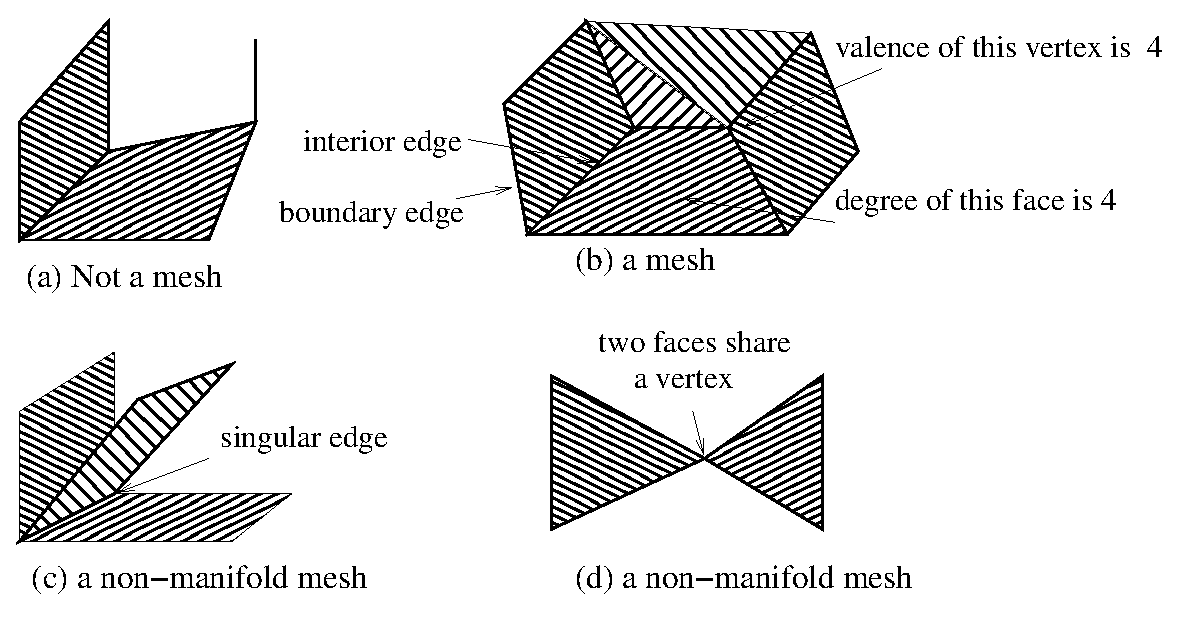
\includegraphics[width=0.8\textwidth]{figure2.1.eps}
\caption[Manifold mesh, non-manifold mesh and non-mesh]{ (a) is not
a mesh since one edge is incident to no face. (b) is a manifold
mesh. (c) is a non-manifold mesh since there is a singular edge.
(d) is a non-manifold mesh since two faces share only a
vertex.\label{mesh_non_mesh}}\
\end{figure}

    Polygonal meshes can be used as an approximation of the surfaces
    of 3D objects. In this case, some properties of the surface such
    as color and normal are often associated with the mesh. These
    properties can be categorized into two types: discrete attributes
    and scalar attributes\label{property}. Discrete attributes, such
    as material identifier, are usually associated with the faces, while
    scalar attributes, such as color, normal, and texture coordinate,
    are often associated with vertices or corners (the tuple (vertex,
    face)). The latter one is used because in the case of
    discontinuity, a vertex can have more than one scalar value. For
    example, if two smooth surfaces intersect at a curve, then vertices
    in this curve will have two different normal values. Therefore,
    the normal value should be associated with the tuple (vertex face).
    Then, polygonal meshes can be represented by $(K, V, D, S)$ where
    $D$ is the set of discrete attributes associated with face $f \in
    K$ and $S$ is the set of scalar attributes associated with corners $(v, f)$ in $S$.

    \section{Coding and Compression}
    A mesh is encoded first before it can be stored or
    transmitted. Coding represents a mesh with a sequence of
    bits. Compression is always combined with coding to save the storage space
    or the bandwidth needed in transmission. 
    There are two kinds of coding:
    single-rate coding and progressive coding. 
    Single-rate coded mesh can only be decoded when all data becomes available 
    whereas progressive coded mesh can be decoded with only part of the data is available. 
    We will briefly introduce single-rate coding methods, and then concentrate on
    progressive coding methods, because the latter are more suitable for progressive streaming.
    
    \subsection{Single-rate Coding} \label{single_rate}
    In a mesh, three kind of information needs to be coded:
    connectivity, geometry and property. 
    Since most property data are associated with vertices, 
    many compression algorithms either treats them as geometry data or 
    ignore them. We first introduce connectivity coding, 
    and then introduce geometry coding briefly.
    
    A triangle mesh is often represented as an array of vertex coordinates
    (geometry information) and an array of triangles (connectivity information). 
    A triangle is represented by the indices of its three vertices,
    where every vertex is indexed by all the
    triangles to which it is incident. Repeated references to the triangles introduce
    redundancy. Such redundancy can be reduced using either 
    %Therefore, triangle strip method is introduced to
    %reduce this redundancy. In a 
    triangle strip, a triangle fan, or a
    generalized triangle strip (a mixture of triangle strips and
    triangle fans) (see Figure \ref{strip}), 
    in which triangles are represented with one index of vertex
    except the first triangle. 
    Deering \cite{218391} first introduced generalized triangular mesh, 
    which combining the generalized triangle strips with a vertex buffer
    to further reduce the bits used to represent indices. 
    Furthermore, Chow \cite{267103} introduced a method to
    decompose a mesh into triangle strips. 
    Bajaj, Pascucci and Zhuang \cite{789628} presented a coding method with layered
    decomposition. 
    Typically, a triangle layer is a generalized triangle strip. 
    \begin{figure}[ht]
    \centering
    \includegraphics[width=0.6\textwidth]{strip.eps}
    \caption{(a) The triangle strip, (b) the triangle fan, and (c) the generated triangle strip.}\label{strip}
    \end{figure}

    Taubin and Rossignac \cite{274365} proposed a method named
    \emph{topological surgery}, which changes coding of a manifold
    mesh to coding of two trees: a vertex spanning tree and the dual of the triangles.
    Topological surgery has been implemented in MPEG-4 standard, and more details
    can be seen in the report of Taubin \cite{3d:Taubin}.
    
    Touma and Gotsman \cite{triangle:Touma} introduced a
    valence-driven approach to encode the connectivity by coding the
    valence of all the vertices in a specific traversing order. 
    The performance is further improved
    by Alliez and Desbrun \cite{alliez01valencedriven}, who also proved a
    upper-bound 3.24 bpv, exactly the theoretical value computed
    by Tutte \cite{census:Tutte} after enumerating all possible planar
    graphs.

    Gumhold and Stra\ss{}er proposed a method called \emph{cut-border machine} \cite{280836}.
    A significant advantage of this method is that it can be easily implemented
    in hardware and the decompression is fast, which
    makes it very useful for real-time coding. 
    Another method named \emph{edgebreaker} is presented by Rossignac \cite{614421}.
    It is similar to the cut-border machine but has better
    compress efficiency and much slower decompression speed.
    
    After introduction of connectivity coding, we briefly introduce geometry
    coding. Most single-rate geometry compression methods involve three steps:
    quantization, prediction, and entropy coding.

    In VRML, geometry data is represented with 32 bit floating-point
    number, but this precision is highly beyond the perceiving
    capability of human eyes. Hence, quantization can be performed to
    compress the geometry data. Typically, each coordinate in a mesh is
    uniformly quantized to 8-16 bits integer.

    After quantization of vertex coordinates, prediction is taken in
    encoding by exploiting correlations between adjacent vertex
    coordinates. An effective prediction scheme generates prediction
    errors with highly compact distribution, which can be effectively
    encoded by entropy coders, such as Huffman coder or arithmetic
    coder. 

    More details about single-rate coding can be seen in the tutorial
    by Gotsman, Gumhold, and Kobbelt \cite{gotsman-simplification},
    the survey by Taubin \cite{3d:Taubin}, by Alliez and Gotsman
    \cite{recent:alliez}, and the survey by Peng, Kim and Kuo
    \cite{technologies:peng}.
    
    \subsection{Progressive Coding}
    (TODO add survey of geometric images)
    Single-rate coded meshes can only be decoded after they are
    completely received, so they are not suitable for streaming. Therefore,
    some progressive coding schemes have been proposed. According to
    how the original mesh is simplified, these coding scheme can be
    categorized into three classes: progressive mesh-based, vertex
    clustering-based, and re-meshing-based.
    
    \begin{description}
        \item[Vertex Clustering-Based] 
            In vertex clustering based schemes, space is divided into cells
            following regular structure such as kd-tree \cite{566591} and 
            octree \cite{1073237}. All vertices inside a cell are represented
            by one delegate. Cells can be further divided into smaller cells
            and the quality of reconstructed model increases. Vertex clustering
            based coding can code geometry information efficiently, but it is 
            difficult to code connectivity information. Moreover, the quality
            of base mesh is poor.

        \item[Re-meshing-Based]
            Re-meshing based method only keeps the shape of a model
            and does not keep the accurate topology. 
            An irregular mesh can be converted into a semi-regular mesh
            with similar shape. 
            %In a semi-regular
            %triangle mesh, the valence of most vertices is six, and therefore
            Because of the regularity of the new mesh,
            the connectivity information can be coded almost without cost.
            More details about these algorithms can be seen in the survey by Allienz and Gotsman
            \cite{recent:alliez}, the survey by Peng, Kim and Kuo
            \cite{technologies:peng} and the references therein.
            Besides losing the correct topology information,
            re-meshing based methods usually code a mesh as a whole, 
            so there is no flexibility in streaming order.

        \item[Progressive Mesh-Based]
            In this thesis, we concentrate on progressive meshes, which provide 
            the finest granularity in choosing streaming order and subset, 
            so we introduce the progressive mesh based coding in more details.
    \end{description}

    The progressive mesh (PM) \label{progressive_mesh}is first
    introduced by Hoppe in 1996 \cite{hoppe96progressive}. In this
    scheme, the simplification is based on \emph{edge collapse}, which
    collapses an edge into a vertex (see Figure \ref{split2}).
    After a series of edge collapse, a coarser \emph{base mesh} remains. 
    Then the PM is constructed by the base mesh and a series of \emph{vertex
    splits}, the inverse of edge collapse, in a reverse order.
    Different level-of-detail can be achieved by applying different number
    of vertex splits.
    %Rendering can be done  n receiver side at any time after the base
    %mesh is received. More vertex splits received, better
    %approximation to the original mesh generated. After all
    %the vertex split operations are received, the original mesh can be
    %reconstructed without loss\footnote{quantization error may exist
    %when quantization is taken in geometry compression.}.

    The base mesh can be encoded with the single-rate coding methods
    introduced in section \ref{single_rate}. Here, we introduce
    how to encode the vertex splits. 
\begin{figure}
\centering
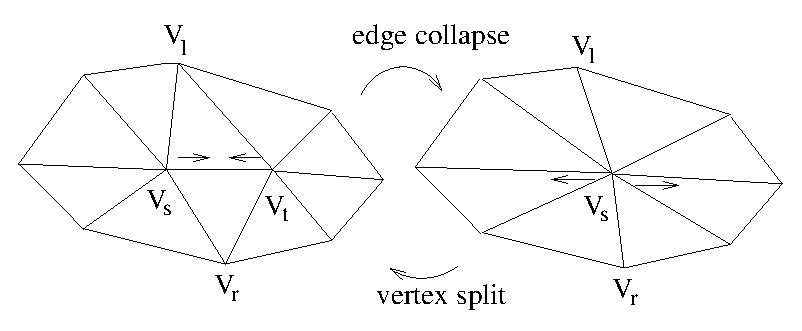
\includegraphics[width=0.5\textwidth]{split2.eps}
\caption{Edge collapse and vertex split}\label{split2}
\end{figure}
    For connectivity
    information, we need to code $s$, $l$, and $r$, and for geometry
    information, we need to code the new position of $v_{s}$ and the
    position of $v_{r}$. If half collapse, which always collapse an
    edge to one of its ends (i.e. $v_{s}$ keeps unchanged), is used, 
    we only need to code the position of $v_r$. 
    
    If the number of vertices in current model is
    $V$, then $s$ can be any one of them, 
    and ${\lceil}log_{2}V{\rceil}$ bits are needed to encode $s$. 
    
    Many compression methods are proposed to reduce this cost.
    Hoppe \cite{efficient:hoppe} present an efficient implementation,
    in which the vertex splits are ordered such that next one
    is as close to current one as possible. This method reduces the cost
    from $O(Vlog_{2}V)$ to $O(V)$.
    Karni, Bogomjakov, and Gotsman \cite{602153}, 
    also use specific order of vertex split to reduce the cost of connectivity. 
    The vertex sequence is generated by recursively cutting a mesh into two
    balanced part with minimum cut. With their algorithm, the connectivity can
    be encoded with in average 4.5 bpv. 

    Another idea is to group many vertex splits together, 
    and efficiency can be improved at the cost of coarser granularity. 
    Taubin, Gu\'{e}ziec, Horn, and Lazarus \cite{280834} proposed the
    progressive forest split scheme (PFS), in which several edge
    collapse operations are combined together and the inverse operation splits a
    forest of edges and vertices. 
    Payarola and Rossignac \cite{614450}, 
    proposed compressed progressive mesh (CPM)\label{cpm} with similar
    idea. They group about $50\%$ vertex splits into one batch. To
    differentiate vertices to be split with others, one bit per vertex
    is used as indicative. 
    Other methods have the similar idea
    but based on vertex removal (remove a vertex and triangulates the hole
    generated) \cite{319358}. 

    More methods exist to reduce the cost in encoding connectivity information.
    Some of them are extended from the single rate coding algorithms
    \cite{319426, 383281}. Some extend progressive mesh to directly
    encode non-manifold meshes \cite{258852}.

    All compression methods introduced above 
    have a common drawbacks. After compression, the 
    data becomes linear and has to be decoded in a fix order. 
    Therefore, these methods improve the coding efficiency at the cost
    of losing flexibility, which is essential in streaming of high-resolution
    progressive meshes.
    
    Flexibility of choosing streaming order 
    is restricted by the dependency among the vertex splits.
    For a manifold mesh, a vertex split operation depends on the existence of
    \begin{itemize}
        \item 
    the vertex to be split ($V_s$ in Figure \ref{split2}), 
        \item 
    two cut neighbors ($V_l, V_r$ in Figure \ref{split2}). 
    \end{itemize}
    More dependencies exist if artificial folds are strictly forbidden \cite{258843, 258847}, 
    but in this thesis we ignore these dependencies since we can 
    tolerate temporary folds in our scheme.
     
    To et al. \cite{To1999} further removed the second dependency.
    In their method, if a cut neighbor does not exist during a vertex split,
    its ancestor are used as the cut neighbor instead.
    Kim and Lee \cite{kim01truly} improved this method so that the final mesh
    can keep the original connectivity. 
    Kim et al. \cite{multiresolution:kim} proposed a better scheme that enables
    an ordinary progressive mesh to be split in random order.

    These methods increase the flexibility, but reduce coding efficiency.
    One solution proposed by Yang et al. \cite{progressive:Yang}
    is to divide the whole mesh into several segments and encode them
    separately to trade off between flexibility and compression efficiency.
    The weakness is that the size of the base mesh is relatively large
    since the original vertices in the border of segments are kept in the base
    mesh. Furthermore, the quality of the base mesh is uneven.

    Kim et al. \cite{multiresolution:kim}
    have proposed a compression algorithm that allows random splitting of a mesh without
    sacrificing compression efficiency. This method is neat since it achieves comparable
    efficiency with other compression methods but maintains the highest flexibility.
    This algorithm, however, is not designed for 
	network transmission.  We extend this algorithm in this thesis. More details are introduced
    in Chapter \ref{c:rdstream}.  
    
    \section{3D streaming}
    \label{s:related:streaming}
    Given the backgrounds in modeling and coding, now we introduce some
    related works in 3D streaming. 
    The main concern in 3D streaming is how to improve the quality of the received
    mesh as fast as possible. Current studies can be categorized into three groups
    by how to achieve this objective.
    %Three main classes of work exist 
    %-- error resilient streaming, packetization, and view-dependent streaming.
    
    \subsection{Error Resilient Streaming}
    To improve the quality quickly, we need to mitigate distortion of the 
    rendered quality of rendered mesh in the presence of packet losses.

    At the transport layer, Al-Regib and Altunbasak \cite{3tpregib}, Li
    et al. \cite{Li2006}, and Chen et al. \cite{chen05hybrid} have
    investigated how to intelligently select either TCP or UDP for
    transmissions to trade off reliability and end-to-end delay.  Li et
    al. have also considered SCTP with partial reliability.
    Harris III and Kravets \cite{harris:design} proposed a new
    transport protocol that exploits loss tolerance and
    partially-ordered property of 3D objects organized into trees of
    bounding volumes.

    At the application layer, the major error control techniques: error
    resilient coding, error protection, retransmission, and error
    concealment \cite{Park2003}, have all been applied to mesh streaming.  
    
    Existing work in robust mesh compression aims to
    reduce dependencies among the mesh \cite{error:Park,error:Yan}.
    Similar to introducing key frames or restart marker in video/image
    coding, mesh segmentation is used to reduce the affected range of one
    packet loss. In robust mesh compression, a mesh is typically
    partitioned into several independent segments and then coded separately.
    Therefore the effect of one packet loss is confined to the segment to which
    it belongs. The finer the partition is, the fewer the affected vertices
    are.  The coding efficiency, however, decreases
    due to more redundancies and less correlation.

    Al-Regib and Altunbasak \cite{unequal:Al-Regib} proposed an
    unequal error protection method to improve the resilience of
    progressive 3D mesh based on CPM (compressed progressive meshes). 
    Forward error correction (FEC) codes are added to the
    base mesh and additional levels-of-detail information to maximize 
    the decoded mesh quality.  The method is similar to FEC protection 
    of video data.

    Chen et al. \cite{chen05hybrid} also applied FEC to streaming
    progressive meshes. They analyzed several transmission schemes:
    TCP only, UDP only, TCP with UDP, and UDP with FEC, and studied
    their effects experimentally on the transmission time and decoded
    mesh quality.

    Cheng et al. \cite{loss:cheng} proposed a sending strategy of mesh
    with textures based on sub-sampling. 
    Their objective is to optimize the perceptional quality, which depends 
    on both geometry quality and texture quality. 
    
    Some studies use retransmission to recover the packet loss.
    For example, Tian \cite{Tian2006} uses selective retransmission in their system.
    We think that retransmission is more suitable than FEC when the feedback
    channel is available, because there is no playback deadline in streaming
    of 3D meshes and data is always useful.

    Most of methods introduced above treat the meshes streamed as 
    traditional linear data. When the flexibility of progressive mesh
    is considered, a new question arises: how to select a sending order
    to improve the quality quickly and mitigate the effect of packet loss.
    We call it the \emph{packetization} problem.
    
    \subsection{Packetization}
    \label{ss:intro:packetization}
    Packetization is tackled by
    Harris III and Karvets in \cite{harris:design}.   
    They proposed a protocol named On-Demand Graphic Transport Protocol (OGP)
    for transmitting 3D models represented as a tree of bounding volumes.
    A key component of the protocol is to decide which bounding volumes
    to send.  OGP begins with packing the largest possible subtree at
    the root and continues to pack the nodes in the subtree of
    acknowledged nodes in breadth-first order.  
    
    Gu and Ooi \cite{Gu:Packetization} were the first to look at
    the packetization problem for progressive meshes.  They model
    the packetization problem as a graph problem where the objective
    is to equally partition the graph into $k$ partitions with minimum
    cut size.  The problem is shown to be NP-complete and a heuristic
    is proposed.  They, however, assume that every vertex split contributes 
    equally to the rendered quality.
    
    In practice, the contribution of vertex splits can
    vary considerably. Therefore, when choosing sending order, we
    need to trade off between minimizing the dependency and sending 
    vertex split with higher contribution first. To achieve this objective,
    the effect of dependency needs to be quantitatively measured.
    There is no existing study is done for this problem
    prior to this thesis.

    A commonly used metric of contribution of vertex splits is 
    Hausdorff distance between the original and reconstructed mesh \cite{cignoni98metro}.
    As Hausdorff distance is view independent, 
    bandwidth may be wasted in sending invisible vertex splits
    before the visible ones. Moreover, even among the visible vertex splits,
    the view-independent metric cannot reflect the real contribution to the visual quality of
    clients with different viewpoints. A vertex split that significantly
    changes a mesh may change the rendered image 
    only slightly.  A better metric for visual contribution of a vertex split,
    based on the rendered image on the screen, 
    needs to consider the receiver's viewpoint.
    Streaming of 3D models based on this metric is named \emph{view-dependent} streaming.

    \subsection{View-Dependent Streaming}
    The view-dependent approach first appeared as 
    a dynamic simplification method used for adaptive rendering of a complex 3D mesh
    \cite{258843, 258847}. Only vertex splits that contribute to the rendered
    image will be rendered, allowing real-time rendering of a complex mesh
    even with limited rendering capability.
    Besides progressive mesh, other multi-resolution representations, 
    such as vertex-clustering  and subdivision scheme,
    are used in view-dependent refinement systems \cite{245627, efficient:Alliez,602344}.

    Later, the view-dependent approach is used in progressive 
	streaming of 3D meshes.     
    In the scheme proposed by Southern et al. \cite{363375},  the client is stateless and
    maintains only the visible data. 
    To et al. \cite{To1999}
    and Kim et al. \cite{kim:view} proposed that received data are stored
    in the receiver even after they become invisible, 
    so they need not be resent when they are visible again. 
    In these papers, view-dependent approaches mainly aim at addressing
    limited rendering capability. 
    
    Yang et al. \cite{progressive:Yang} and
    Zheng et al. \cite{zheng:interactive}, on the other hand, use
    view-dependent streaming to address limited network bandwidth.
    Yang et al. proposed a scheme where the server chooses the appropriate resolution
    according to the available network bandwidth.
    Zheng et al. \cite{zheng:interactive} use prediction to
    reduce the effect of network latency and 
    compensate the round-trip delay with the rendering time.
    Moreover, Yang et al. \cite{optimized:yang} proposed an joined 
    optimizing transmission method based on a general rate-distortion
    model that considers both mesh and texture data. Their method
    allocates bits between mesh and texture to optimize the display 
    quality at every stage of progressive transmission.
     
    These systems use sender-driven approach and do not address
    server scalability issues. Due to the stateful design, 
    the sender-driven approach is difficult to be extended to
    support caching proxy and peer-to-peer techniques, two 
    common solutions to scalability. This thesis presents the first
    scalable 
    view-dependent streaming system without incurring high infrastructural cost.
    

